% Capítulo 4 - Metodologia
% Implementação
% deve constar o instrumental, os métodos e as técnicas aplicados para a elaboração do trabalho;

\abrv[MBRPSOLA -- \emph{Multi-Band Resynthesis Pitch Synchronous Overlap and Add}]
\simb[ms (milissegundos)]
\simb[Hz (Hertz)]
\abrv[API -- \emph{Application Programming Interface}]
\abrv[JSON -- \emph{JavaScript Object Notation}]
\abrv[REST -- \emph{Representational State Transfer}]
\abrv[AJAX -- \emph{Asynchronous JavaScript And XML}]

\chapter{Módulo de prosódia}
Baseado na revisão da literatura, decidiu-se criar um módulo de prosódia que
permite anotações prosódicas manuais, tornando possível variar a prosódia
afetiva e aumentativa para um sistema TTS.

\section{Implementação}
\subsection{espeak-ng}
Foi utilizado o programa \emph{open-source} eSpeakNG \cite{espeakng} para
realizar as primeiras etapas do \emph{front end}: normalização de texto e
conversão grafema-fone, ou seja, obter a partir do texto de entrada uma
representação em fones. A saída gerada pelo programa é subsequentemente passada
para o programa desenvolvido neste trabalho através da biblioteca
\code{subprocess} da linguagem Python. O comando utilizado para obter os
fones pode ser visto na Figura \ref{lst:espeak}.

\begin{itemize}
\item A \emph{flag} \code{-v} seleciona uma voz. Neste caso, \code{pt-br}.
\item \code{-x} e \code{-q} escrevem fones na saída em vez da fala sintetizada.
\item \code{-sep=/} separa fones utilizando o caractere \code{/}.
\item O caractere \code{\'} indica \emph{primary stress}, ou seja, o fone tônico
da palavra.
\end{itemize}

\begin{figure}[thp]
    \centering
    \begin{tabular}{c}
        \begin{lstlisting}
        $ espeak-ng -v pt-br 'Bom dia' -x -q --sep=/
        $ b/'o/N dZ/'i/&
        \end{lstlisting}
    \end{tabular}
    \caption{Utilização do programa espeak e saída correspondente \label{lst:espeak}}
\end{figure}

Apesar da existência de outras ferramentas para \emph{front end} para o
português brasileiro, optamos pelo eSpeakNG pela disponibilidade e facilidade de
instalação.
% O sistema TTS desenvolvido por \citeonline{couto} não foi encontrado para \emph{download} no início de desenvolvimento deste trabalho.

% MBROLA usa interpolação linear, INTSINT sugere quadratic spline

\subsection{MBROLA}
O programa \code{sampa_mbrola.py} foi desenvolvido para converter a saída gerada
pelo eSpeakNG mostrada anteriormente em fones possíveis de serem sintetizados
pela voz utilizada no \emph{back end}. O equivalente ao fone \code{/&/} gerado
pelo espeak é \code{/a/} na voz do MBROLA, por exemplo.

A ferramenta de conversão lê a tabela do arquivo \code{sampa_mbrola.tbl} e
substitui cada fone em notação XSAMPA pelo equivalente. A tabela possui três
colunas: o fone que o espeak produz, o fone equivalente para o MBROLA e um
exemplo numa palavra do português. Na Figura \ref{sampambrola} é possível ver
algumas linhas do arquivo. Utilizamos neste trabalho a voz \code{br3}
desenvolvida por Denis R. Costa disponível no site oficial do projeto MBROLA.

\begin{figure}[thp]
    \centering
    \begin{tabular}{c}
        \begin{lstlisting}
        b  |  b  | _b_arco
        k  |  k  | _c_om
        d  |  d  | _d_ose
        &  |  a  | v_a_le
        6  |  @  | tam_a_nho
        n  |  n  | _n_unca
        \end{lstlisting}

    \end{tabular}
    \caption{Extrato de linhas da tabela de conversão \label{sampambrola}}
\end{figure}

Além da conversão XSAMPA-MBROLA, são determinadas as durações padrão para cada
fone a partir da Tabela \code{durations.tbl}, adaptada do código utilizado pelo
LianeTTS \cite{lianetts}. Cada linha contém o fone e uma duração em milissegundos.

\subsection{INTSINT}
\label{intsintrules}
Como visto na seção \ref{intsintsec}, o INTSINT serve não apenas para análise,
mas também para síntese de contornos $ f_0 $. Escolhemos utilizá-lo na implementação
pela simplicidade da notação e flexibilidade.

Em \code{intsint.py} (Figura \ref{intsintpy}) é feita a determinação de valores $ f_0 $ a partir do texto de
entrada anotado e das regras descritas na Tabela \ref{tab:intsint}. O
algoritmo \ref{alg:intsint} ilustra o funcionamento do processo de conversão.

\begin{algorithm}[H]
\begin{algorithmic}
  \REQUIRE{lista de rótulos P, $ \forall i : P_i \in \{ T, M, B, H, S, L, U \}$}
  \ENSURE{lista de frequências f (em Hertz)}
\STATE freq\_t $ \gets \text{key} \times \sqrt{2^{range}}$
\STATE freq\_m $ \gets \text{key} $
\STATE freq\_b $ \gets \text{key} / \sqrt{2^{range}} $
\IF {rótulo $ P_0 \notin \{ T, M, B \} $}
\STATE retorne erro \COMMENT{Primeiro rótulo deve ser absoluto}
\ENDIF
\FORALL {rótulo $ P_i $}
  \IF {$ P_i $ = T}
    \STATE $ f_i \gets $ freq\_t
  \ELSIF {$ P_i $ = M}
    \STATE $ f_i \gets $ freq\_m
  \ELSIF {$P_i$ = B}
    \STATE $ f_i \gets $ freq\_b
  \ELSIF {$ P_i $ = H}
  \STATE $ f_i \gets \sqrt{f_{i - 1} \times \text{freq\_t}} $
  \ELSIF {$ P_i $ = S}
    \STATE $ f_i \gets f_{i - 1} $
  \ELSIF {$ P_i $ = L}
  \STATE $ f_i \gets \sqrt{f_{i - 1} \times \text{freq\_b}} $
  \ELSIF {$ P_i $ = U}
  \STATE $ f_i \gets \sqrt{f_{i - 1} \times  \sqrt{f_{i - 1} \times \text{freq\_t}}} $
  \ELSIF {$ P_i $ = D}
  \STATE $ f_i \gets \sqrt{f_{i - 1} \times  \sqrt{f_{i - 1} \times \text{freq\_b}}}  $
  \ENDIF
\ENDFOR
\end{algorithmic}
\caption{Pseudocódigo para geração de frequências utilizando modelo INTSINT \label{alg:intsint}}
\end{algorithm}

% \subsection{Módulo de prosódia}
% O programa foi codificado utilizando a linguagem de programação Python 3.6,
% calculando contorno $ f_0 $ a partir de notação especificada pelo usuário seguindo o
% modelo INTSINT. O módulo é uma interface entre os programas eSpeakNG e MBROLA,
% calculando parâmetros a partir da representação textual inicial e sua conversão
% em fones geradas pelo \emph{front end}, calculando valores de duração para cada
% fone a partir de uma tabela e gerando frequências a partir do algoritmo
% encontrado na seção \ref{intsintrules}.

\subsection{Editor gráfico}
Para permitir refinamento de prosódia após cálculo inicial de parâmetros, foi
desenvolvido um editor gráfico para \emph{web} utilizando HTML, CSS e
JavaScript. A duração e altura de cada fone podem ser especificadas manualmente
arrastando barras de controle, gerando um novo arquivo de áudio com a fala
sintetizada a partir dos novos parâmetros.

\subsubsection{Arquitetura}
 O editor se comunica com o espeak-ng e MBROLA através de um
servidor programado em Python utilizando o \emph{framework} Flask para prover
\emph{endpoints} de uma API \emph{RESTful}. Foi utilizada uma arquitetura
cliente-servidor \cite{rest} comumente observada em aplicações \emph{web}
atuais. A maneira como os módulos se comunicam pode ser vista na Figura
\ref{fig:arch}. Os módulos implementados neste trabalho estão com bordas
espessas.

\begin{figure}[!htbp]
\centering
\scalebox{0.80}{
    \begin{tikzpicture}[auto, >={Latex[inset=0pt, length=3mm, angle'=28,round]}, box/.style={draw,rounded corners,text width=3.0cm,align=center}]
    \node[] (txt) {Texto};
    \node[box, right=of txt] (esp)
        {eSpeakNG};
    \node[box, right=of esp, line width=1.6pt] (con)
        {Conversão eSpeakNG para MBROLA};
    \node[box, right=of con, line width=1.6pt] (sin)
        {Gerador de $ f_0 $ por INTSINT};
    \node[above=of con] (ano)
        {Texto anotado};

    \node[box, below=of sin, line width=1.6pt] (ser)
        {Servidor};

    \node[box, left=of ser] (mbr)
        {MBROLA};

    \node[box, below=of ser, line width=1.6pt] (int)
        {Interface gráfica};

    \draw[->] (ano) -| (txt);
    \draw[->] (ano) -- (con);
    \draw[->] (txt) -- (esp);
    \draw[->] (esp) -- (con);
    \draw[->] (con) -- (sin);

    \draw[->] (sin) -- (ser);
    \draw[->] (mbr) -- (ser);

    \draw[<->] (ser) -- (int);

    \end{tikzpicture}
}
\caption{Arquitetura para o programa da interface gráfica \label{fig:arch}}
\end{figure}

\subsubsection{\emph{Endpoints}}
Foram criados dois \emph{endpoints} para a API, possibilitando a comunicação entre
interface gráfica e servidor.

\paragraph{[POST] /api/espeak} Recebe um texto como entrada e gera uma resposta
no formato JSON com lista de fones. Cada fone, por sua vez, possui campos \code{duration},
\code{phone_mbrola}, \code{phone_sampa} e \code{pitch_changes}. Um exemplo de resposta pode ser visto na Figura \ref{espeakpost}.
\paragraph{[POST] /api/mbrola} Recebe uma lista de fones no formato MBROLA
descrito na seção \ref{sec:mbrola}, passa a lista para o programa para criar o
arquivo de áudio final e gera uma resposta com o nome do arquivo de áudio
contendo a fala sintetizada.
\subsection{Utilização}
O programa pode ser executado através de uma interface de linha de comandos,
como ilustrado na Figura \ref{cmdline}.

\begin{figure}[thp]
    \centering
    \begin{tabular}{c}
        \begin{lstlisting}[language=Python]
        $ echo "Testando" | python3 sampa_mbrola.py > out.pho
        $ mbrola ../br3/br3 out.pho out.wav; afplay out.wav
        \end{lstlisting}

    \end{tabular}
    \caption{Utilização por linha de comandos \label{cmdline}}
\end{figure}
Alternativamente, pode-se utilizar um navegador e ter acesso à interface
gráfica descrita anteriormente e vista na Figura \ref{fig:ed}, permitindo
edição de parâmetros para fones individuais.

\begin{figure}[!htbp]
  \centering
    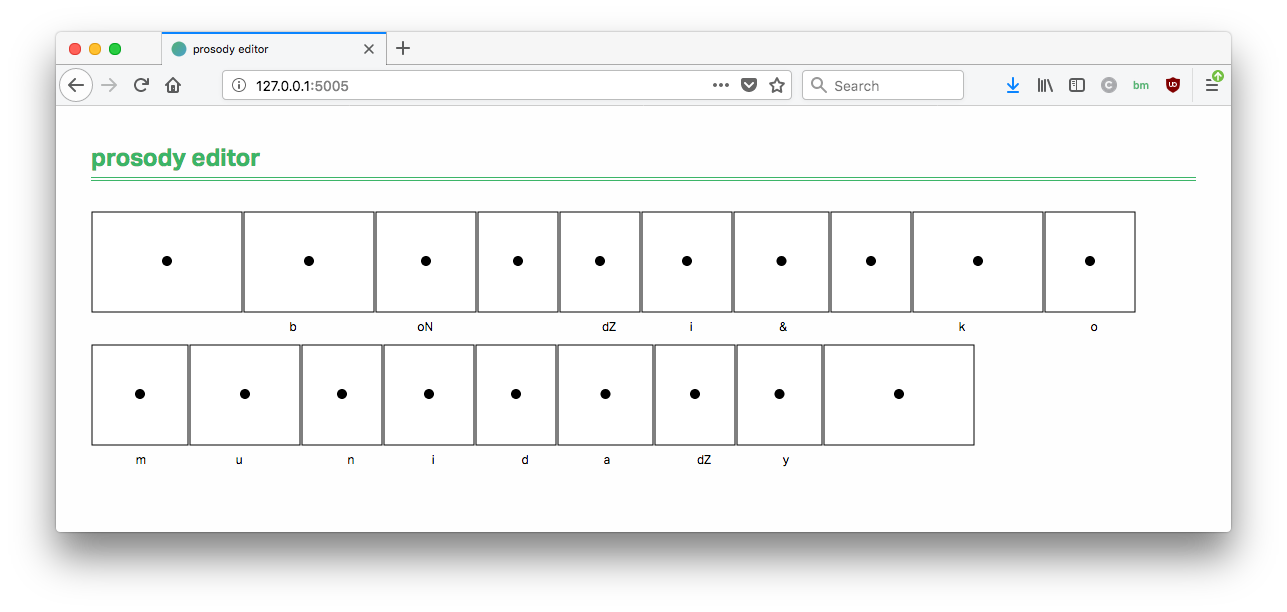
\includegraphics[width=1.0\textwidth]{Imagens/editor.png}
  \caption{Editor gráfico desenvolvido \label{fig:ed}}
\end{figure}


% A interface gráfica é uma aplicação \emph{web}
% Também foi desenvolvido um editor gráfico para permitir refinamento do contorno melódico
% gerado pelo algoritmo de \citeonline{intsintalg}.

% \begin{figure}[!htbp]
% \centering
% \scalebox{0.65}{
%     \begin{tikzpicture}[auto, >={Latex[inset=0pt, length=3mm, angle'=28,round]}, box/.style={draw,rounded corners,text width=3.0cm,align=center}]
%     \node[] (txt) {Texto};
%     \node[box, right=0.7cm of txt] (pre)
%         {Pré-processador};
%     \node[box, right=0.2cm of pre] (mor)
%         {Analisador morfológico};
%     \node[box, right=0.2cm of mor] (con)
%         {Analisador de contexto};
%     \node[box, right=of con] (let)
%         {Módulo letra-som};
%     \node[box, right=of let] (pro)
%         {Gerador de prosódia};
%         
%     \draw[->] (txt) -- (pre);
%         
%     \node[box, fit=(pre)(mor)(con), label={[name=morfos_l] Analisador morfossintático}] (morfos) {};
%     \node[box, fit=(let)] (letsom) {};
%     \node[box, fit=(pro)] (proger) {};
%     
%     \node[inner sep=0, fit=(morfos)(letsom)(proger)] (all) {};
%     \node[box,
%           inner sep=0,
%           yshift=-0.75cm,
%           fit=(morfos.west)(proger.east),
%           label=center:Estrutura de dados,
%           minimum height=1cm,
%           below of=all]
%         (dad) {};
%     
%     \node[box, fit=(morfos)(morfos_l)(letsom)(proger)(dad), label=Processamento de linguagem natural] (nlp) {};
%     
%     \node[right=of dad, align=left] (out) {\emph{phones}\\ prosódia};
%     
%     \draw[->] (pre) -- (pre |- dad.north);
%     \draw[<->] (mor) -- (mor |- dad.north);
%     \draw[<->] (con) -- (con |- dad.north);
%     \draw[<->] (let) -- (let |- dad.north);
%     \draw[<->] (pro) -- (pro |- dad.north);
%     
%     \draw[->] (dad) -- (out);
%         
%     \end{tikzpicture}
% }
% \caption{Arquitetura de um sistema de geração de prosódia}
% \label{fig:nlpdiagram}
% \end{figure}
